\begin{frame}{NICE: Non-linear Independent Components Estimation}

Unsupervised Learning
    \begin{itemize}
        \item Capture complex unknown data distributions
        \item Data representation task
        \begin{itemize}
            \item Idea: Map data into a latent space so that the resulting distribution is factorial
        \end{itemize}
    \end{itemize}

\begin{align*}
h &= f(x)    \\
p_H(h) &= \prod_d p_{h_d}(h_d)
\end{align*}
\end{frame}
\begin{frame}{NICE: Change of variable rule}
$f$ is invertible and dimensionality of $h$ is the same as $x$
\begin{align*}
    p_X(x) = p_H(f(x))|\text{det}\frac{\partial f(x)}{\partial x}|
\end{align*}
$\frac{\partial f(x)}{\partial x}$ is the Jacobian of $f$.
\newline
\newline
Given that $f$ is invertible, we can sample from $p_X(x)$ by:
\begin{align*}
    h \sim p_H(h)\\
    x = f^{-1}(h)
\end{align*}
KEY contribution: $f$ with easy inverse and determinant of Jacobian
\end{frame}
\begin{frame}{NICE: Core idea}
\begin{itemize}
\item Learn the probability density over a dataset $\mathcal{D} \in \mathbb{R}^D$
\item By learning a continuous, differentiable transformation $f$ of the data distribution into a \textit{simpler} distribution.
\item Use maximum likelihood using the change of variable formula
\begin{align*}
    log(p_X(x)) = log(p_H(f(x))) + log(|\text{det}\frac{\partial f(x)}{\partial x}|)
\end{align*}
\item $p_H(h$) is a \textit{prior} distribution, e.g. Gaussian or Logistic
\item If $p_H$ is factorial, i.e. has independent dimensions:
\begin{align*}
    log(p_X(x)) = \sum_{d=1}^{D} log(p_{H_d}(f_d(x))) + log(|\text{det}\frac{\partial f_d(x)}{\partial x}|)
\end{align*}
\end{itemize}
\end{frame}
\begin{frame}{NICE: Architecture}
\begin{itemize}
    \item Use a layered transformation
    \begin{align*}
        f = f_L \circ \dots \circ f_2 \circ f_1
    \end{align*}
    \item The Jacobian determinant is the product of the Jacobian determinant of its layers.
    \item Calculating the determinant has $\mathcal{O}(D^3)$ cost, so...
    \item Find $f_i$ with tractable determinants
    \begin{itemize}
        \item Triangular matrices: determinant is the product of the diagonal elements
    \end{itemize}
\end{itemize}
\end{frame}

\begin{frame}{NICE: General coupling layer}
    \begin{itemize}
        \item Create a partition of $x \in \mathbb{R}^D$ using $I_1 = [1, d]$ and $I_2 = [d, D]$
        \item Define $y = (y_{I_1}, y_{I_2})$
            \begin{align*}
                y_{I_1} &= x_{I_1} \\
                y_{I_2} &= g(x_{I_2}; m(x_{I_1}))
            \end{align*}
        \item $m : \mathcal{R}^d \longrightarrow \mathcal{R}^{D-d}$, e.g. a NN with $d$ inputs and $D-d$ outputs.
        \item Coupling law \\
        $g : \mathcal{R}^{D-d} \times m(\mathcal{R}^d) \longrightarrow \mathcal{R}^{D-d}$
        \item The Jacobian is $\frac{\partial y}{\partial x} =$
        $\begin{bmatrix}
            I_1 & 0 \\
            \frac{\partial y_{I_2}}{\partial x_{I_1}} &  \frac{\partial y_{I_2}}{\partial x_{I_2}}
        \end{bmatrix}$
        \item And since $I_1$ is an identity matrix of size $d$: $\frac{\partial y}{\partial x} = \frac{\partial y_{I_2}}{\partial x_{I_2}}$
    \end{itemize}
\end{frame}

\begin{frame}{NICE: Additive coupling layer}
\begin{itemize}
    \item Additive coupling law: $g(a; b) = a + b$
    \begin{align*}
                y_{I_1} &= x_{I_1} \\
                y_{I_2} &= x_{I_2} + m(x_{I_1})
    \end{align*}
    \item Inverse
    \begin{align*}
                x_{I_1} &= y_{I_1} \\
                x_{I_2} &= y_{I_2} - m(x_{I_1})
    \end{align*}
    \item Jacobian determinant
    \begin{align*}
        \text{det} \; \frac{\partial y_{I_2}}{\partial x_{I_2}} = 1
    \end{align*}
\end{itemize}
\end{frame}

\begin{frame}{NICE: layered architecture and scaling}
    \begin{itemize}
        \item By composing several layers, a more complex transformation can be obtained.
        \item The coupling layer leaves a part of the input unchanged
        \begin{itemize}
            \item Exchange the role of the two subsets in alternating layers
        \end{itemize}
        \item Additive coupling layers have volume preserving determinants.
        \item To allow scaling, use a diagonal scaling matrix $S$ at the top layer.
        \begin{itemize}
            \item Allows the learner to assign more weights to some dimentions than others
        \end{itemize}
        \begin{align*}
            log(p_X(x)) = \sum_{i=1}^D[log(p_{H_i}(f_i(x)))+log(|S_{ii}|)]
        \end{align*}
    \end{itemize}
\end{frame}
\begin{frame}{NICE: Architecture example}
\begin{align*}
    h_{I_1}^{(1)} &= x_{I_1}\\
    h_{I_2}^{(1)} &= x_{I_2} + m^{(1)}(x_{I_1})\\ 
    h_{I_2}^{(2)} &= h_{I_2}^{(1)}\\
    h_{I_1}^{(2)} &= h_{I_1}^{(1)} + m^{(2)}(x_{I_2})\\ 
    h_{I_1}^{(3)} &= h_{I_1}^{(2)}\\
    h_{I_2}^{(3)} &= h_{I_2}^{(2)} + m^{(3)}(x_{I_1})\\ 
    h_{I_2}^{(4)} &= h_{I_2}^{(3)}\\
    h_{I_1}^{(4)} &= h_{I_1}^{(3)} + m^{(4)}(x_{I_2})\\ 
    h &= \text{exp}(s) \odot h^{(4)}
\end{align*}
\end{frame}
\begin{frame}{NICE: Prior distributions}
    \begin{itemize}
        \item Gaussian
        \begin{align*}
            log(p_H(h)) = -\frac{1}{2}(h_d^2 + log(2\pi))
        \end{align*}
        \item Logistic
        \begin{align*}
            log(p_H(h)) = - log(1+exp(h_d)) - log(1+exp(-h_d))
        \end{align*}
    \end{itemize}
\end{frame}
\begin{frame}{NICE: Experiments}
    \begin{itemize}
        \item Datasets
        \begin{itemize}
            \item MNIST
            \item Toronto Face Dataset (TFD)
            \item Street View House Numbers (SVHN)
            \item CIFAR-10
        \end{itemize}
        \item Adam optimizer
            \begin{itemize}
                \item learning rate = 0.001 
                \item momentum = 0.9 
                \item $\beta_2$ = 0.01 
                \item $\lambda$ = 1 
                \item $\epsilon$ = 0.0001 
            \end{itemize}
        \item Data whitening preprocessing
        \item All $m$ coupling functions are deep rectified networks with linear outputs
    \end{itemize}
\end{frame}
\begin{frame}{NICE: Results}
    \begin{figure}
        \centering
        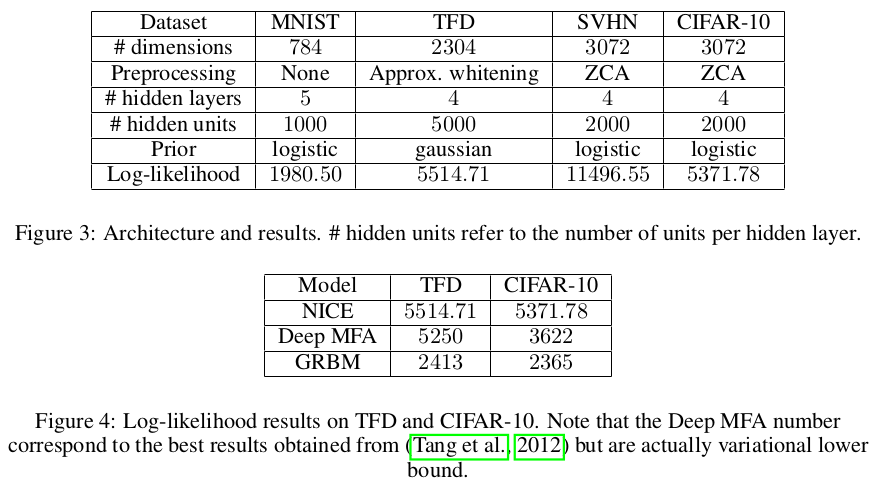
\includegraphics[width=\textwidth]{Images/nice_experiments.png}
        \label{fig:nice_params_results}
    \end{figure}
\end{frame}
\begin{frame}{NICE: Results}
    \begin{figure}
        \centering
        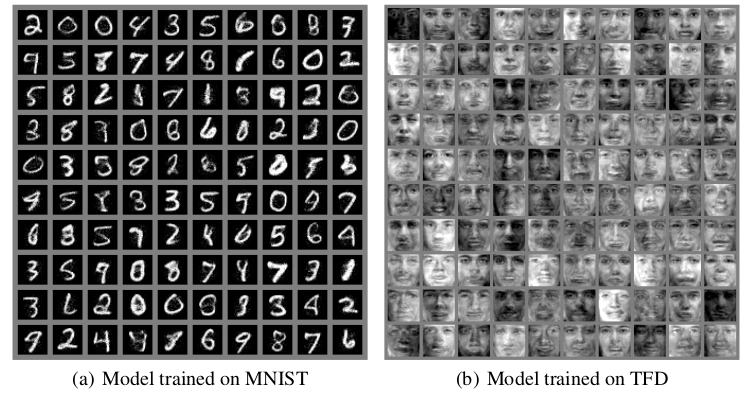
\includegraphics[width=\textwidth, height = 8cm, keepaspectratio]{Images/nice_sampling_1.png}
        \label{fig:nice_sampling}
    \end{figure}
\end{frame}
\begin{frame}{NICE: Results}
    \begin{figure}
        \centering
        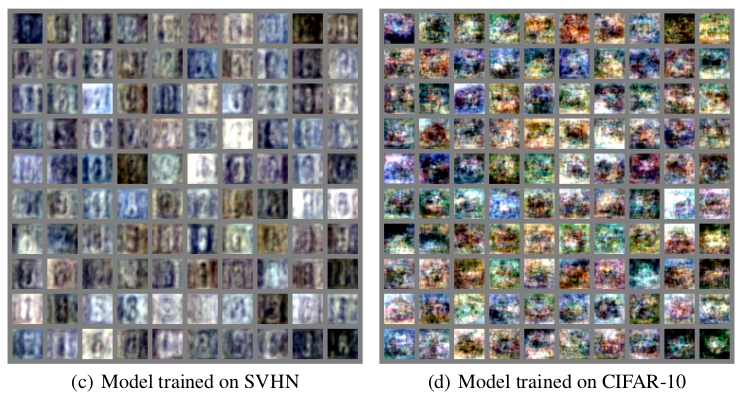
\includegraphics[width=\textwidth, height = 8cm, keepaspectratio]{Images/nice_sampling_2.png}
        \label{fig:nice_sampling2}
    \end{figure}
\end{frame}
